\documentclass{article}
\usepackage{graphicx}
\usepackage{multicol} % use to multiple column in itemize
\usepackage{float}
\usepackage{setspace}
\setlength{\parskip}{0.5em}

\begin{document}

\title{Logistic Regression}
\author{Cong Cuong PHAM}

\maketitle

\begin{abstract}
This document introduces some fundamental notions of Logistic Regression.
\end{abstract}

\section{Introduction}
\subsection{What is Logistic Regression?}
\par Logistic Regression is a method for {\bf{Classification}}. Examples: Spam versus ``Ham'' emails; Loan defaults, Disease Diagnosis...

\par Logistic Regression allows to solve classification problems, where we are trying to predict discrete categories (although we have continuous value). The convention for {\bf{binary classification}} is to have two classes 0 and 1.

\par We can't use a normal linear regression model on binary groupes. It won't lead to a good fit:

\begin{figure}[H]
\centering
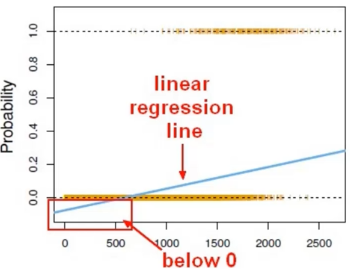
\includegraphics[width=.6\linewidth]{pic/linear_regression-binary_classification.png}
\caption{The linear regression is not suitable for the binary classification.}
\end{figure}

\par We can transform our linear regression to a logistic regression curve. The Sigmoid (aka Logistic) Function takes in any value and ouputs it to be between 0 and 1 (Figure \ref{sigmoid-function}).

\begin{figure}[H]
\centering
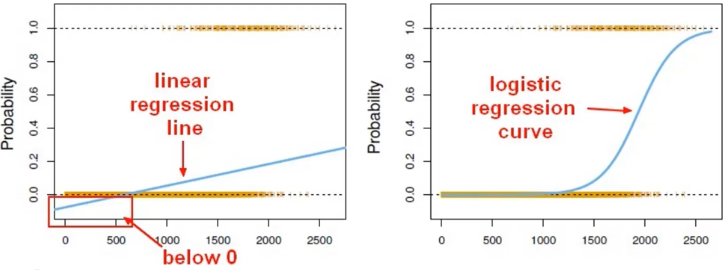
\includegraphics[width=\linewidth]{pic/linear-logistic_regression.png}
\caption{Linear and logistic regression.}
\end{figure}

\begin{figure}[H]
\centering
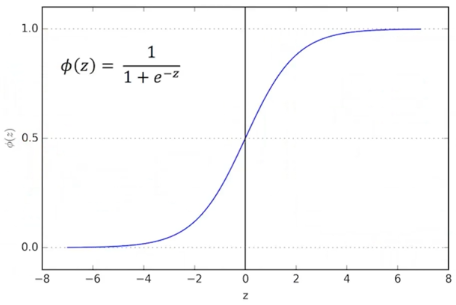
\includegraphics[width=.6\linewidth]{pic/sigmoid-function.png}
\caption{Sigmoid (aka Logistic) function.}
\label{sigmoid-function}
\end{figure}

\begin{figure}[H]
\centering
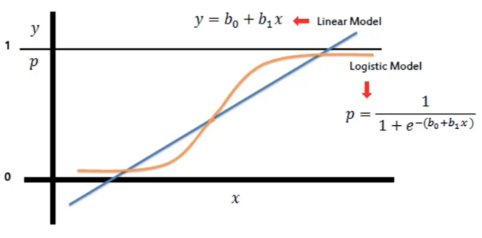
\includegraphics[width=.8\linewidth]{pic/linear_regression-sigmoid_function.png}
\caption{Linear Regression Solution used Sigmoid Function.}
\end{figure}

\par After training a logistic regression model on some training data, you will evaluate your model's performance on some test data. A {\bf{confusion matrix}} (Figure \ref{confusion-matrix}) could be used to evaluate classification models. 

\begin{figure}[H]
\centering
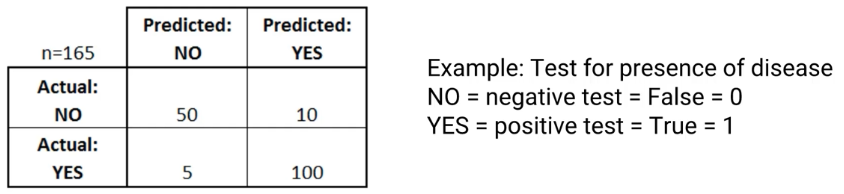
\includegraphics[width=.9\linewidth]{pic/confusion-matrix.png}
\caption{Confusion matrix used to evaluate classification models.}
\label{confusion-matrix}
\end{figure}

\begin{figure}[H]
\centering
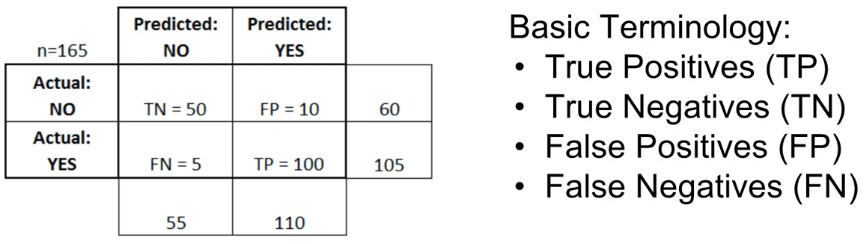
\includegraphics[width=.9\linewidth]{pic/confusion-matrix2.png}
\caption{Confusion matrix - F value.}
\label{confusion-matrix2}
\end{figure}

\begin{figure}[H]
\centering
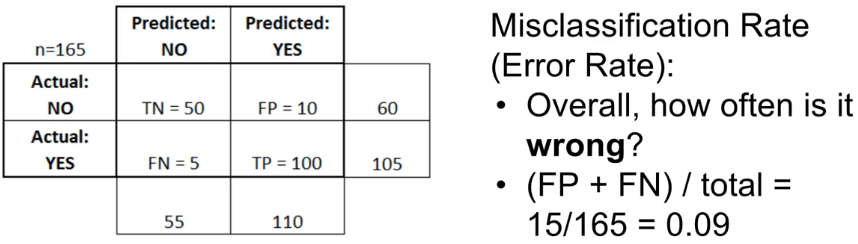
\includegraphics[width=.9\linewidth]{pic/confusion-matrix3.png}
\caption{Confusion matrix - Misclassification Rate.}
\label{confusion-matrix3}
\end{figure}

\begin{figure}[H]
\centering
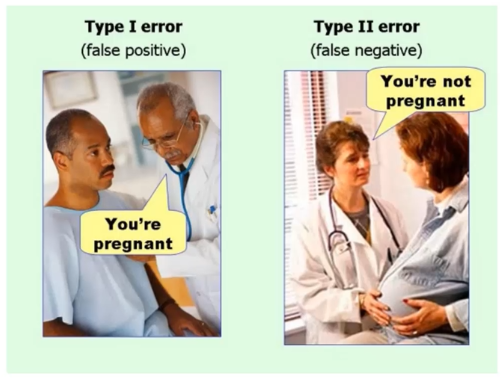
\includegraphics[width=.9\linewidth]{pic/confusion-matrix4.png}
\caption{Confusion matrix - Misclassification Rate - Example.}
\label{confusion-matrix4}
\end{figure}

\end{document}